%-------------------------------------------
\begin{frame}{Workflow definition}
%-------------------------------------------
%\begin{block}{Linked commands}
 a pool of commands, progressively linked by the treatments of the input data towards the results:\\
    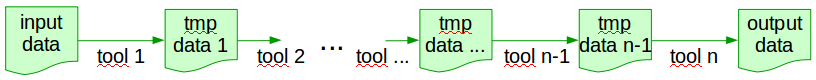
\includegraphics[width=12cm]{03_workflow/images/FAIR_smk_data_wf.png}\\
   arrow: output of tool $n-1$ = input for tool $n$
%\end{block}
\begin{block}{How to save time?}
Improve algorithms? Are we ready to optimize Bowtie2? hem ... no!\\
With multiple data for analysis $\Rightarrow$ we can parallelize.
\end{block}
\end{frame}
%-------------------------------------------
\begin{frame}{Data parallelization}
%-------------------------------------------
%\begin{block}{Time saving}
  Several data flows can be processed in parallel:
  \begin{center}
     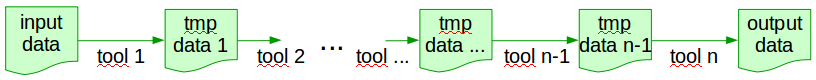
\includegraphics[width=12cm]{03_workflow/images/FAIR_smk_data_wf.png}\\
     $\Downarrow$\\
     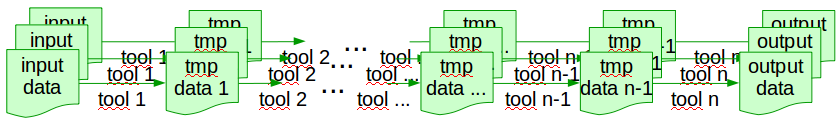
\includegraphics[width=12cm]{03_workflow/images/FAIR_smk_n_data_wf.png}
  \end{center}
  With a multi-cores PC or a computational cluster (ex. 2000 cores), we can attribute one core to one workflow.
%\end{block}
\end{frame}
%-------------------------------------------
%\begin{frame}{A workflow is launched. How to reduce the waiting time?}
%-------------------------------------------
%    Improve algorithms? Are we ready to optimize Bowtie2? hem ... no!\\
%    We have multiple data and steps of analyses $\Rightarrow$ we can parallelize!\\
%    \begin{center}
%            \includegraphics[height=6cm]{03_workflow/images/FAIR_WF_linear_vs_parallel_en.png}
%    \end{center}
%\end{frame}
%-------------------------------------------
\begin{frame}{Workflow management system}
%-------------------------------------------
Many workflow management systems, many forms:
\begin{itemize}
    \item command line: shell (but doesn't handle parallelization alone, need to script it, not easy)
    \item rule: \includegraphics[height=1cm]{shared/logo-snakemake.png}, \includegraphics[height=0.5cm]{shared/logo-cmake.png}, \logoNextflow, ...
    \item graphic interface: Galaxy, Taverna, Keppler, ...
\end{itemize}
\vfill
pros: important for reproducibility (keep track of when each file was generated, and by which operation), manage parallelization\\
cons: learning effort
\vfill
We choose \includegraphics[height=1cm]{shared/logo-snakemake.png}
\end{frame}
%-------------------------------------------
\begin{frame}[containsverbatim]
\frametitle{Snakemake rule}
%-------------------------------------------
Snakemake: mix of the programming language Python (snake) and the rule-based automation tool Make\footnote{Make: https://www.gnu.org/software/make/manual/}\\
Good practice: one step, one rule
\begin{block}{A rule is defined by it name and may contain:}
\begin{itemize}
    \item \verb|input:| list one or more file names
    \item \verb|output:| list one or more file names
    \item command (\verb|run:| for python ; \verb|shell:| for shell, R, etc)
\end{itemize}
+ optional directives: \verb|params:|, \verb|message:|, \verb|log:|, ...\\
Remark: with 1 command line, use a \verb|shell:| directive ; with many command lines, use a \verb|run:| directive with python shell("...") functions.
\end{block}
\begin{center}
    \includegraphics[height=1.8cm]{03_workflow/images/FAIR_WF_rule_concept_en.png}
\end{center}
\end{frame}
%-------------------------------------------
\begin{frame}[containsverbatim]
\frametitle{Hello World example}
%-------------------------------------------
The objective of this example is to write "Hello World" into the file \verb|world.txt| in the directory \verb|hello|:
\begin{block}{hello$\_$world.smk:}
\begin{lstlisting}
rule hello_world:
    output: "hello/world.txt"
    shell: "echo Hello World > hello/world.txt"
\end{lstlisting}
 % docker run -v ${PWD}:/home -w /home snakemake/snakemake snakemake -j1 --snakefile helloworld.smk 
\end{block}
\begin{itemize}
    \item this rule contains only an \verb|output:| directive (\verb|echo| command construction)
\end{itemize}
\end{frame}
%-------------------------------------------
\begin{frame}{Snakemake}
%-------------------------------------------
Snakemake automatically makes sure that everything is up to date, otherwise it launch the jobs that need to be.
\vfill
Snakemake:
\begin{itemize}
    \item works on files (rather than streams, reading/writing from databases or passing variables in memory)
    \item is based on Python (but know how to code in Python is not required to work with Snakemake)
    \item has features for defining the environment with which each task is carried out (running a large number of small third-party tools is current in bioinformatics)
    \item is easily to be scaled from desktop to server, cluster, grid or cloud environments (ie. develop on laptop using a small subset of data, run the real analysis on a cluster)
\end{itemize}    
\end{frame}
%-------------------------------------------
\begin{frame}{Data flow linkage}
%-------------------------------------------
A snakemake workflow links rules thank to the filenames of the rule input and output directives:
\begin{center}
    \includegraphics[height=1.8cm]{03_workflow/images/FAIR_WF_rule_concept_en.png}\includegraphics[height=1.8cm]{03_workflow/images/FAIR_signeEgal.png}\includegraphics[height=1.8cm]{03_workflow/images/FAIR_WF_rule_concept_en.png}
\end{center}
\begin{block}{Snakemake rules order:}
   the first rule (all, target, ...) specifies the result files, the next rules describe how to achieve them.
\end{block}
\end{frame}
%-------------------------------------------
\begin{frame}[containsverbatim]
\frametitle{Rule execution order}
%-------------------------------------------
Snakemake starts with the first rule that describes the workflow result files. Since output files do not exist, it "goes back" through the workflow until it finds a file to apply a rule to. 
\begin{center}
    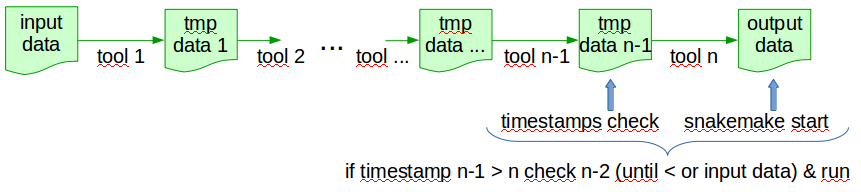
\includegraphics[width=12cm]{03_workflow/images/FAIR_smk_wf_timestamps.png}
\end{center}
For determining whether output files have to be re-created, Snakemake checks whether the file modification date (i.e. the timestamp) of any file is newer than the timestamp of the output file.
\end{frame}
%-------------------------------------------
\begin{frame}[containsverbatim]
\frametitle{Generalization with wilcards}
%-------------------------------------------
Wildcards (a Snakemake key feature) allow to replace part of filenames:
\begin{itemize}
    \item reduce hardcoding: more flexible input and output directives, work on new data without modification
    \item are writing into \verb|{}| 
    \item are automatically resolved (ie. replaced by regular expression \verb|".+"| in filenames)
\end{itemize}
Wildcards are specific to a rule, a same file can be accessed by different matching:
\begin{block}{Ex. with the file "101$/$file.A.txt"}
\begin{lstlisting}
rule one: output: "{set}1/file.{grp}.txt" => set=10, grp=A
rule two: output: "{set}/file.A.{ext}" => set=101, ext=txt
\end{lstlisting}
\end{block}
\vfill
(more on \href{https://snakemake.readthedocs.io/en/stable/snakefiles/rules.html#wildcards}{\textcolor{blue}{\underline{wildcards}}} in the snakemake documentation)
\end{frame}
%-------------------------------------------
\begin{frame}[containsverbatim]
\frametitle{With and without wilcards examples}
%-------------------------------------------
\begin{block}{without$\_$wildcards$\_$uniprot.smk}
\begin{lstlisting}
rule all:
 input: "P10415.fasta", "P01308.fasta"

rule get_prot:
 output: "P10415.fasta", "P01308.fasta"
 run:
  shell("wget https://www.uniprot.org/uniprot/P10415.fasta")
  shell("wget https://www.uniprot.org/uniprot/P01308.fasta")
\end{lstlisting}
\end{block}
% bel exemple issu de https://endrebak.gitbooks.io/the-snakemake-book
% mais ping n'étant pas présent par défaut dans le docker snakemake 
% => remplacement par uniprot
%rule all:
%  input: "ping/github.txt", "ping/duckduckgo.txt"
%rule ping:
% output: "ping/github.txt", "ping/duckduckgo.txt
% run:
%  shell("ping -c3 github.com > ping/github.txt")
%  shell("ping -c3 duckduckgo.com > ping/duckduckgo.txt")
%
%rule ping:
% output: "ping/{host}.txt"
% run:
%  shell("ping -c3 {wildcards.host}.com > ping/{wildcards.host}.txt")
\begin{block}{with$\_$wildcards$\_$uniprot.smk}
\begin{lstlisting}
rule get_prot:
  output: "{prot}.fasta"
  run:
    shell("wget https://www.uniprot.org/uniprot/{wildcards.prot}.fasta")
\end{lstlisting}
\end{block}
\end{frame}
%-------------------------------------------
\begin{frame}[containsverbatim]
\frametitle{Input (output) specifications}
%-------------------------------------------
\begin{block}{enumerated}
\begin{lstlisting}
rule one:
  input: "P10415.fasta", "P01308.fasta"
\end{lstlisting}
\end{block}
\begin{block}{python list $\&$ wildcards}
\begin{lstlisting}
DATASETS = ["P10415", "P01308"]
rule one: 
  input: ["{dataset}.fasta".format(dataset=dataset) 
          for dataset in DATASETS] 
\end{lstlisting}
\end{block}
\begin{block}{expand() $\&$ wildcards}
\begin{lstlisting}
DATASETS = ["P10415", "P01308"]
rule one: 
  input: expand("{dataset}.fasta", dataset=DATASETS) 
\end{lstlisting}
\end{block}
\end{frame}
%-------------------------------------------
\begin{frame}[containsverbatim]
\frametitle{Snakemake accesses}
%-------------------------------------------
\begin{block}{Laptop with docker}
\begin{lstlisting}[language=bash]
docker pull snakemake/snakemake  #install (linux: add sudo)
docker run -v ${PWD}:/data -w /data snakemake/snakemake snakemake ...  #run
\end{lstlisting}
\end{block}
\begin{block}{Laptop with conda}
\begin{lstlisting}[language=bash]
conda create -n smk-env -c bioconda snakemake  #install
conda activate smk-env ; snakemake ...         #run
\end{lstlisting}
\end{block}
\begin{block}{IFB core cluster}
\begin{lstlisting}[language=bash]
module load snakemake ; snakemake ...           #run
\end{lstlisting}
\end{block}
check run: replace \verb|...| by \verb|--version|
\end{frame}